\makeatletter{}\RequirePackage{fix-cm}
\documentclass[smallextended]{svjour3}

\usepackage{booktabs}
\usepackage{subcaption}
\usepackage{comment}
\usepackage{mathrsfs}
\usepackage{balance}
\usepackage{enumitem}
\usepackage{hyperref}
\usepackage[noend]{algpseudocode}
\usepackage[group-separator={,}]{siunitx}
\usepackage{caption}
\usepackage{mathtools}
\usepackage{amssymb}
\usepackage{amsfonts}
\usepackage{listings}
\usepackage{algorithm}
\usepackage{algorithmicx}
\usepackage{bm}
\usepackage[all]{hypcap}
\usepackage[absolute]{textpos}
\usepackage{wrapfig}
\usepackage[title]{appendix}


\renewcommand{\algorithmicrequire}{\textbf{Input:}}
\renewcommand{\algorithmicensure}{\textbf{Output:}}
\algnewcommand{\LineComment}[1]{\State{\(\triangleright\) #1}}
\newcommand*\Let[2]{\State #1 := #2}

\smartqed

\usepackage{graphicx}
\graphicspath{{./figures/}}


\hypersetup{  bookmarks=true,
  unicode=true,
  pdftoolbar=true,
  pdfmenubar=true,
  pdffitwindow=true,
  pdfstartview={FitV},
  pdfnewwindow=true,
  colorlinks=false,
  pdfdisplaydoctitle=true,
  pdfborder={0 0 0}
}

\setlength{\TPHorizModule}{1in}
\setlength{\TPVertModule}{1in}
\textblockorigin{0.75in}{0.875in}

\setlist[itemize]{leftmargin=*,partopsep=5pt}
\setlist[enumerate]{leftmargin=*,partopsep=5pt}

\paperheight 11in
\paperwidth 8.5in

\usepackage{dcolumn}
\newcolumntype{d}[1]{D{.}{.}{#1}}

\newcommand\nil{\textit{nil}}

\usepackage{tikz}
\newcommand*\circled[1]{\tikz[baseline=(char.base)]{
      \node[shape=circle,draw,inner sep=0pt] (char) {#1};}}

\makeatletter
\newcommand*{\rome}[1]{\expandafter\@slowromancap\romannumeral #1@}
\makeatother

\makeatletter{}
\newcommand{\wifi}{Wi-Fi}
\newcommand{\codename}{\textsc{Verifier}}
\newcommand{\us}{$\mu$s}
\newcommand{\ns}{\textsc{NS-3}}

\newcommand{\shuvendu}[1]{{\bf [[SKL:{#1}]]}}
 

 

\def\thetitle{Wireless Protocol Validation Under Uncertainty}
\def\theauthors{}

\authorrunning{J. Shi, S. K. Lahiri, R. Chandra, G. Challen}

\journalname{Formal Methods in System Design}

\begin{document}

\title{  \thetitle\thanks{This work was published, in part, in Runtime Verification
    (RV) 2016~\cite{Shi2016}.}
}

\author{  Jinghao Shi$^1$ \and
  Shuvendu K. Lahiri$^2$ \and
  Ranveer Chandra$^2$ \and
  Geoffrey Challen$^1$
}

\institute{
  Jinghao Shi\\
  jinghaos@buffalo.edu\\\\
  Shuvendu K. Lahiri\\
  shuvendu@microsoft.com\\\\
  Ranveer Chandra\\
  ranveer@microsoft.com\\\\
  Geoffrey Challen\\
  challen@buffalo.edu\\\\
  $^1$University at Buffalo, Buffalo, NY 14260, USA\\
  $^2$Microsoft Research, Redmond, WA 98052, USA
}

\hypersetup{  pdfinfo={    Title={\thetitle},
    Author={\theauthors},
  }
}


\maketitle

\makeatletter{}\begin{abstract}
  Runtime validation of wireless protocol implementations cannot always employ
  direct instrumentation of the device under test (DUT). The DUT may not
  implement the required instrumentation, or the instrumentation may alter the
  DUT's behavior when enabled. Wireless sniffers can monitor the DUT's
  behavior without instrumentation, but they introduce new validation challenges.
  Losses caused by wireless propagation prevent sniffers
  from perfectly reconstructing the actual DUT packet trace. As a result,
  accurate validation requires distinguishing between
  specification deviations that represent implementation errors and those
  caused by sniffer uncertainty.

  \sloppy{
  We present a new approach enabling sniffer-based validation of wireless
  protocol implementations. Beginning with the original protocol monitor state
  machine, we automatically and completely encode sniffer uncertainty by
  selectively adding non-deterministic transitions. We characterize the
  NP-completeness of the resulting decision problem and provide an exhaustive
  algorithm for searching over all mutated traces. We also present
  practical protocol-oblivious heuristics for searching over the most likely
  mutated traces.  We have implemented our framework and show that it can
  accurately identify implementation errors in the face of uncertainty.
}
  
  \keywords{
    Runtime Verification \and
    Wireless Protocol \and
    Sniffer \and
  Uncertainty}
\end{abstract}
 
\makeatletter{}\section{Introduction}
\label{sec:intro}

Custom wireless protocols are often designed and deployed to meet the specific
performance and power needs of special-purpose wireless devices. Examples
include Google
Iris contact lenses~\cite{iris}, Xbox One wireless controllers~\cite{xbox}, and
Google Chromecast~\cite{chromecast}. Validating that device implementations work
correctly is critical to achieve the design goals of the wireless protocol and
also prevent bugs in shipped products~\cite{wifried,lollipop,surface}.


Runtime validation of the protocol implementations on such devices is
challenging because collecting traces from the device under test (DUT) is often
infeasible. The resource limitations of embedded or battery-powered devices may
cause them to not provide trace collecting capabilities. DUT may contain
proprietary hardware or firmware that hides the implementation details and
prevents testers from collecting traces through source code instrumentation.
Even when collecting trace directly from the DUT is possible, the overhead it causes
may alter the behavior of the DUT due to the observer
effect~\cite{mytkowicz2008observer}, threatening the validation results.

An attractive alternative is to use wireless
sniffers to record traffic generated by the DUT during testing.
Sniffers do not require direct access to the DUT or the need to alter its behavior.
However, due to the fundamentally unpredictable nature of wireless
communications, the packets captured by the sniffer will not exactly match
those received by the DUT.
The sniffer may miss packets that the DUT received, or receive packets that
the DUT missed.
This is true even when using multiple
sniffers~\cite{cheng2006jigsaw,mahajan2006analyzing,bahl2006enhancing}, a sniffer
with multiple antennas~\cite{omnipeek}, or in isolated wireless environments.

Since the sniffer trace may not perfectly match the actual trace, uncertainty
arises during protocol implementation validation.  For example, if the DUT fails
to respond correctly to a packet in the sniffer trace, it may either because the
DUT's implementation is incorrect, or the DUT did not actually receive the
packet, or the DUT's response was missed by the sniffer.  Whenever the DUT's
behavior does not match the specification, there are now two potential
explanations: either the DUT's implementation is wrong, or the sniffer trace is
inaccurate. Accurate validation requires  distinguishing between these two
causes.

We present a new technique than enables validation of protocol implementations using
wireless sniffers. Given a monitor state machine representing the protocol being
validated, we describe a systematic transformation that adds non-deterministic
transitions to incorporate uncertainty introduced by the sniffer. This
augmented validation state machine implicitly defines a set of
mutated traces, each satisfying the original state machine with a specific
likelihood. If the set is empty, the implementation definitely violates the
protocol. Searching over all the mutated traces is NP-complete, but the approach
can be made practical by applying protocol-oblivious heuristics that limit the
search to likely mutated traces.

Our paper makes the following contributions:
\begin{enumerate}
  \item To the best of our knowledge, we are the first to identify the
    uncertainty problem caused by sniffers in validating wireless protocol
    implementations.
  \item We formalize the problem using a nondeterministic state machine that
    systematically and completely encodes the uncertainty of the
    sniffer trace.
  \item We characterize the NP-completeness of the validation problem, and
    present two protocol-oblivious heuristics to prune the search space and make
    validation possible in practice.
  \item We implement the validation framework and evaluate it using the \ns{}
    network simulator~\cite{riley2010ns}. Our framework accurately identifies
    both synthetic and previously unknown violations in \ns{}'s implementations
    of the 802.11 and ARF protocols.  We also applied our framework to a
    commercial product under development and was able to found three latent bugs
    that were not observed previously.
\end{enumerate}

This paper is an extension of our work that appeared in RV 2016~\cite{Shi2016}.
We added the proof for Lemma~\ref{lem:mutation}, \ref{lem:sub} and
Theorem~\ref{the:equivalent}. We included new results that show the searching
cost (Fig.~\ref{fig:cost}), and details of the ARF protocol violations
(Section~\ref{subsec:arf}). Further, we reported the application of our
framework to a commercial product under development in
Section~\ref{subsec:xbox}.
 
\makeatletter{}\section{Background and Motivating Example}
\label{sec:motivation}

We encountered the uncertainty problem while testing the protocol implementation
of a popular wireless game controller. A custom wireless protocol
was designed to meet the low latency and low power consumption goals. As is
common industry practice, the protocol specification was then handed over to
wireless chipset vendors for implementation. However, neither implementation
details nor trace collection capabilities are provided in the shipped firmware
due to intellectual property constraints and device resource limitation. Hence
using sniffers to validate the protocol implementation is the only option.

We initially developed a tool to validate certain protocol properties over the
sniffer trace, yet often found unacceptable amount of false alarms due to
the incompleteness of the sniffer traces, making the tool virtually useless. It
was clear that we needed to account for sniffer uncertainty.

\begin{figure}[t!]
  \centering
  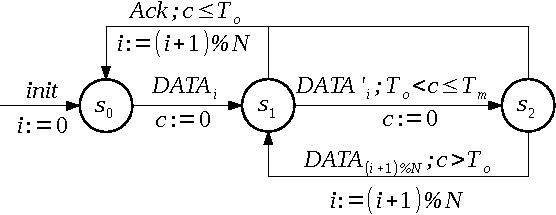
\includegraphics[width=0.6\textwidth]{dot11_tx_ta.pdf}
  \caption{\textbf{Monitor State Machine for 802.11 Transmitter.}}
  \label{fig:dot11_tx_ta}
\end{figure}


To better understand the incompleteness of sniffer trace, consider the IEEE
802.11 (also known as \wifi{}) transmitter (DUT) state machine shown in
Fig.~\ref{fig:dot11_tx_ta}. After the DUT sends $\it{DATA}_i$---a data packet with
sequence number $i$ ($s_0\rightarrow s_1)$, it starts a timer and waits for the
acknowledgment packet---$Ack$. The DUT either receives $Ack$ within time $T_o$
($s_1\rightarrow s_0$), or it sends $\it{DATA}'_i$---retransmission of $\it{DATA}_i$
($s_1\rightarrow s_2$). Similarly, the DUT either receives the $Ack$ within $T_o$
($s_2\rightarrow s_0$) or aborts transmission and moves on to next
packet\footnote{To represent the state machine succinctly, our example assumes
that the DUT retries at most once.} ($s_2\rightarrow s_1$).


Given a complete log of DUT's packet transmission and reception events, it is
trivial to feed such a log into the state machine in Fig.~\ref{fig:dot11_tx_ta}
and validate the correctness of DUT's protocol implementation. However, due to
DUT limitations we have described earlier, this complete log is not
available. As a result, we seek to validate the DUT implementation using
sniffers.

There are two fundamental properties in wireless communication that bring uncertainty to
sniffer's observation: packet loss and physical diversity. The sniffer could
either miss packets sent from or to the DUT due to packet loss, or overhear packets
that are sent to but missed by the DUT due to physical diversity.

\begin{figure}[t!]
  \centering
  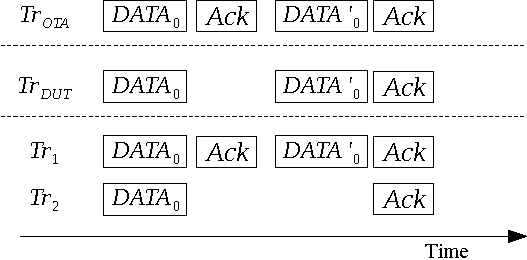
\includegraphics[width=0.6\textwidth]{false_pos.pdf}
  \caption{\textbf{Uncertainty of Sniffer Observations.} $Tr_{OTA}$ is
    the chronological sequence of packets sent by the DUT and the receiver.
    $Tr_{DUT}$ is DUT's internal events. $Tr_1$ and $Tr_2$ are two examples of
    many possible sniffer traces.}
  \label{fig:sniffer_in_middle}
\end{figure}

Consider a correct packet exchange sequence shown in
Fig.~\ref{fig:sniffer_in_middle}. The DUT first sends $\it{DATA}_0$.  Suppose the
receiver receives $\it{DATA}_0$ and sends the $Ack$ which the DUT does not receive.
Eventually the DUT's timer fires and it sends $\it{DATA}'_0$.  This time the
$\it{DATA}'_0$ reaches receiver and the DUT also receives the $Ack$.

Now consider two possible traces that could have been overheard by a sniffer shown
in Fig.~\ref{fig:sniffer_in_middle}.
In first sniffer trace $Tr_1$ where the sniffer
\textit{overhears} the first $Ack$ packet, a validation \textit{uncertainty}
arises when the sniffer sees the $\it{DATA}'_0$: was the previous $Ack$ missed by the
DUT or is there a bug in DUT which causes it to retransmit even after receiving
the $Ack$?

Similarly, consider the second possible sniffer trace $Tr_2$
where both the $\it{DATA}'_0$ and $Ack$ packets were missed by the sniffer. During
this period of time, it appears the DUT neither receives $Ack$ for $\it{DATA}_0$ nor
sends $\it{DATA}'_0$. Again, without any additional information it is impossible to
disambiguate between the sniffer missing certain packets and a bug in DUT's
retransmission logic.

Informally, the question we set out to answer in this paper is: given the
protocol monitor state machine and the sniffer's observation with inherent
uncertainty, how to accurately validate that the DUT behaves as specified?
 
\makeatletter{}\section{Prerequisites and Problem Statement}
\label{sec:background}

\subsection{Packet, Trace and Monitor State Machine}
\label{subsec:basic}

The alphabet of the monitor state machine is the finite set of all valid packets
defined by the protocol, denoted as $\mathbb{P}$.  A packet is a binary string
of a finite number of bits, encoding interesting protocol attributes such as
\texttt{src}, \texttt{dest}, \texttt{type}, \texttt{flags}, and physical layer
information, such as \texttt{channel}, \texttt{modulation}, etc. The input of
the state machine then corresponds to a time-ordered sequence of packets.

\begin{definition}[Packet Trace]
  \sloppy{
  A \textit{packet trace} is a finite sequence of $(timestamp, packet)$ tuple:
  $[(t_1, p_1), (t_2, p_2),\ldots,(t_n, p_n)]$ where $t_i \in \mathbb{Z}^+$ is
  the \textit{discrete} timestamp and $p_i$ is the packet observed at time
  $t_i$. The timestamps are strictly monotonically increasing: $t_i < t_{i+1}$
  for $1 \le i < n$.
}
\end{definition}
In addition to timestamp monotonicity, we also require that adjacent packets do
not overlap in time, $t_{i+1}-t_i > \text{\texttt{airtime}}(p_i)$ for $1 \le i <
n$, where \texttt{airtime()} calculates the time taken to transmit a packet.
The timestamp represents the observer's local clock ticks, and need not to be
synchronized among devices.

We use \textit{timed automata}~\cite{alur1994theory} to model the expected
behaviors of the DUT. A timed automata is a finite state machine with timing
constraints on the transitions: each transition can optionally start one or more
timers, which can later be used to assert certain events should be seen before
or after the time out event. We refer the readers to~\cite{alur1994theory} for
more details about timed automata.


\begin{definition}[Monitor]
  \sloppy{    A protocol monitor state machine $S$ is a 7-tuple
    $\{\Sigma, \mathbb{S}, \mathbb{X}, s_0, C, E, G\}$, where:
  }
  \begin{itemize}
    \item $\Sigma = \mathbb{P}$ is the finite input alphabet.

    \item $\mathbb{S}$ is a non-empty, finite set of states. $s_0 \in
      \mathbb{S}$ is the initial state.

    \item $\mathbb{X}$ is the set of boolean variables. We use $v = \{x
      \leftarrow true/false\ |\ x \in \mathbb{X}\}$ to denote an assignment of
      the variables. Let $\mathbb{V}$ be the set of such values $v$. 

    \item $C$ is the set of clock variables. A \textit{clock variable} can be
      reset along any state transitions. At any instant, reading a clock
      variable returns the time elapsed since last time it was reset.

    \item $G$ is the set of guard conditions defined inductively by
      \begin{align*}
        g := true\ |\ c \le T\ |\ c \ge T\ |\ x\ |\ \neg g\ |\ g_1 \land g_2
      \end{align*}      where $c \in C$ is a clock variable, $T$ is a constant, and $x$ is a
      variable in $\mathbb{X}$.  A transition can choose not to use guard
      conditions by setting $g$ to be $true$.

    \item $E \subseteq \mathbb{S} \times \mathbb{V} \times \mathbb{S} \times
      \mathbb{V} \times \Sigma \times  G \times \mathscr{P}(C)$ gives the set of
      transitions.\\ $\langle s_i, v_i, s_j, v_j, p, g, C'\rangle \in E$
      represents that if the monitor is in state $s_i$ with variable assignments
      $v_i$, given the input tuple $(t, p)$ such that the guard $g$ is
      satisfied, the monitor can transition to a state $s_j$ with variable assignments
      $v_j$, and reset the clocks in $C'$ to 0.
  \end{itemize}
  \label{def:sm}
\end{definition}

A tuple $(t_i, p_i)$ in the packet trace means the packet $p_i$ is presented to
the state machine at time $t_i$. The monitor {\it rejects a trace} $Tr$ if there
exists a prefix of $Tr$ such that all states reachable after consuming the
prefix have no valid transitions for the next $(t, p)$ input.

As an example, the monitor state machine illustrated in
Fig.~\ref{fig:dot11_tx_ta} can be formally defined as follows:

\begin{itemize}
  \item $\Sigma = \{\it{DATA}_i, \it{DATA}'_i, Ack\ |\ 0 \le i < N\}$.
  \item Clock variables $C = \{c\}$. The only clock variable $c$ is
    used for acknowledgment time out.
  \item $\mathbb{X} = \{i\}$, as a variable with ${\mathit log}(N) + 1$ bits to
    count from $0$ to $N$.  
  \item Guard constraints $G = \{ c \le T_o, c > T_o, T_o < c \le T_m\}$.
    $T_o$ is the acknowledgment time out value, and $T_m >
    T_o$ is the maximum delay allowed before the retransmission packet gets
    sent. $T_o$ can be arbitrary large but not infinity in order to check the
    liveness of the DUT.
\end{itemize}


The monitor state machine defines a \textit{timed language} $L$ which consists
of all valid packet traces that can be observed by the DUT.  We now give the
definition of protocol \textit{compliance} and \textit{violation}.

\begin{definition}[Violation and Compliance]
  Suppose $\mathbb{T}$ is the set of all possible packet traces collected from
  DUT, and $S$ is the state machine specified by the protocol. The DUT
  \textit{violates} the protocol specification if there exists an
  packet trace $Tr \in \mathbb{T}$ such that $S$ rejects $Tr$.
  Otherwise, the DUT is \textit{compliant} with the specification.
\end{definition}

The focus of this paper is to determine whether a \textit{given} sniffer trace
$Tr$ is evidence of a violation.


\subsection{Mutation Trace}
\label{subsec:mutation}

As shown in the motivation example in Fig.~\ref{fig:sniffer_in_middle}, a
sniffer trace may either miss packets that are present in DUT trace, or contain
extra packets that are missing in DUT trace. Note that in the latter case, those
extra packets must be all sent \textit{to} the DUT. This is because it is
impossible for the sniffer to overhear packets sent from the DUT that were not
actually sent by the DUT.

We formally capture this relationship with the definition of mutation trace.

\begin{definition}[Mutation Trace]
  \label{def:mutation}
  A packet trace $Tr'$ is a mutation of sniffer trace $Tr$ w.r.t a DUT if for
  all $(t, p) \in Tr \setminus Tr'$, $p.dest = DUT$, where $p.dest$ is the
  destination of packet $p$.
\end{definition}

By definition, either $Tr' \supseteq Tr$ (hence $Tr \setminus Tr' = \emptyset$),
or those extra packets in $Tr$ but not in $Tr'$ are all sent to the DUT. Note
that $Tr'$ may contain extra packets that are either sent to or received by
the DUT.

A mutation trace $Tr'$ represents a \textit{guess} of the corresponding DUT
packet trace given sniffer trace $Tr$.  In fact, the DUT packet trace must
be one of the mutation traces of the sniffer trace $Tr$.

\begin{lemma}
  Let $Tr_{DUT}$ and $Tr$ be the DUT and sniffer packet trace captured during
  the same protocol operation session, and $\mathcal{M}(Tr)$ be the set of
  mutation traces of $Tr$ with respect to DUT, then $Tr_{DUT} \in \mathcal{M}(Tr)$.
  \label{lem:mutation}
\end{lemma}\begin{proof}
  Let $\Delta = Tr \setminus Tr_{DUT}$ be the set of packets that are in $Tr$
  but not in $Tr_{DUT}$. Recall that it is not possible for the sniffer to
  observe packets sent from the DUT that the DUT did not send. Therefore,
  all packets in $\Delta$ are sent \textit{to} the DUT. That is, for
  all $(t, p) \in \Delta,\ p.dest = DUT$. By Definition~\ref{def:mutation},
  $Tr_{DUT} \in \mathcal{M}(Tr)$.
  \qed
\end{proof}


\subsection{Problem Statement}
\label{subsec:problem}

Lemma~\ref{lem:mutation} shows that $\mathcal{M}(Tr)$ is a \textit{complete} set
of guesses of the DUT packet trace. Therefore, the problem of validating DUT
implementation given a sniffer trace can be formally defined as follows:

\begin{problem}
  \label{prob:validation}
  VALIDATION\\
  \textbf{instance} A protocol monitor state machine $S$ and a sniffer trace $Tr$.\\
  \textbf{question} Does there exist a mutation trace $Tr'$ of $Tr$ that satisfies $S$?
\end{problem}

If the answer is no, a definite violation of the DUT implementation can be
claimed. Nevertheless, if the answer is yes, $S$ may still reject $Tr_{DUT}$.
In other words, the conclusion of the validation can either be
\textit{definitely wrong} or \textit{probably correct}, but not
\textit{definitely correct}.  This is the fundamental limitation caused by the
uncertainty of sniffer traces.
 
\makeatletter{}\section{Validation Framework}
\label{sec:framework}

\makeatletter{}\subsection{Augmented State Machine}
\label{subsec:augment}

To deal with the inherent uncertainty of sniffer traces, we propose to
systematically augment the original monitor state machine with non-deterministic
transitions to account for the difference between the sniffer and DUT traces.


Before formally defining the augmented state machine, we first use an example to
illustrate the basic idea. Fig.~\ref{fig:augment} shows the augmented state
machine for 802.11 transmitter state machine shown in
Fig.~\ref{fig:dot11_tx_ta}.  For each existing transition (e.g., $s_0\rightarrow
s_1$), we add an \textit{empty transition} with same clock guards and resetting
clocks.  This accounts for the possibility when such packet was observed by
the DUT but missed by the sniffer.  Additionally, for each transition triggered
by a \textit{receiving} packet (i.e., $p.dest = DUT$), such as $s_1\rightarrow
s_0$ and $s_2\rightarrow s_0$, we add a \textit{self transition} with the same
trigger packet and clock guards, but an empty set of resetting clocks and no
assignments to variables. This allows the state machine to make progress when
the sniffer missed such packets.

\begin{figure}[t!]
  \centering
  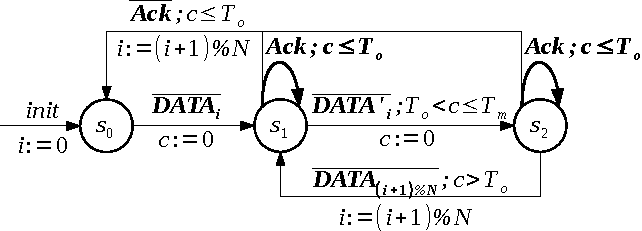
\includegraphics[width=0.7\textwidth]{dot11_tx_checker.pdf}
  \caption{\textbf{Augmented Monitor State Machine.} Augmented transitions are
  highlighted in bold face. $\overline{Pkt}$ means either $\epsilon$ or $Pkt$.}
  \label{fig:augment}
\end{figure}


There are two things to note. First, self transitions are added only for
packets sent \textit{to} the DUT, since the sniffer will not overhear packets
\textit{from} the DUT if they were not sent by the DUT. Second, no augmented
transitions are added for the packets that are sent to DUT yet are missed by both
the DUT and the sniffer, since such packets do not cause difference between the
DUT and sniffer traces.

The augmented state machine in Fig.~\ref{fig:augment} will accept the sniffer
packet traces $Tr_1$ and $Tr_2$ shown in Fig.~\ref{fig:sniffer_in_middle}.  For
instance, one accepting transition sequence on sniffer trace $Tr_1$ is
$s_0\rightarrow s_1 \rightarrow_s s_1\rightarrow s_2 \rightarrow s_0$, and the
sequence for $Tr_2$ is $s_0 \rightarrow s_1 \rightarrow_e s_2 \rightarrow s_0$,
where $\rightarrow$ is the transition from the original state machine,
$\rightarrow_e$ and $\rightarrow_s$ are the augmented empty and self transitions
respectively.

We now formally define the augmented state machine.

\begin{definition}[Augmented Monitor]
  \sloppy{
  An augmented state machine $S^+$ for a monitor state machine $S$ is a 7-tuple
  $\{\boldsymbol{\Sigma^+}, \mathbb{S}, \mathbb{X}, s_0, C, \boldsymbol{E^+},
  G\}$, where $\mathbb{S}, \mathbb{X}, s_0, C, G$ are the same as $S$.
  $\Sigma^+=\{\epsilon\} \cup \Sigma$ is the augmented input alphabet with the
  empty symbol, and $E^+ \supset E$ is the set of transitions, which includes:
}
  \begin{itemize}
    \item $E$: existing transitions (\textbf{Type-0}) in $S$.
    \item $E^+_1$: empty transitions (\textbf{Type-1}) for transitions in $E$.
    \item $E^+_2$: self transitions \textbf{(Type-2)} for transitions
      triggered by receiving packets.
  \end{itemize}
\end{definition}

\begin{figure}[t!]
\begin{algorithm}[H]
  \caption{Obtain Augmented Transitions $E^+$ from $E$}
  \label{alg:augment}
  \begin{algorithmic}[1]
    \Function{augment}{$E$}
    \Let{$E^+$}{$\emptyset$}
    \ForAll{$\langle s_i, v_i, s_j, v_j, p, g, C'\rangle \in E$}
      \Let{$E^+$}{$E^+ \cup \{\langle s_i, v_i, s_j, v_j, p, g, C'\rangle\}$\Comment{Type-0}}
      \label{alg:augment:type0}
      \Let{$E^+$}{$E^+ \cup \{\langle s_i, v_i, s_j, v_j, \boldsymbol{\epsilon}, g, C'\rangle\}$\Comment{Type-1}}
      \label{alg:augment:type1}
      \If{$p.dest = DUT$}
      \Let{$E^+$}{$E^+ \cup \{\langle s_i, v_i, \boldsymbol{s_i},
      \boldsymbol{v_i}, p, g, \boldsymbol{\emptyset}\rangle\}$\Comment{Type-2}}
        \label{alg:augment:type2}
      \EndIf
    \EndFor
    \State \Return{$E^+$}
    \EndFunction
  \end{algorithmic}
\end{algorithm}
\end{figure}

Algorithm~\ref{alg:augment} describes the process of transforming $E$ into
$E^+$. In particular, Line~\ref{alg:augment:type0} adds existing transitions in
$E$ to $E^+$, while line~\ref{alg:augment:type1} and~\ref{alg:augment:type2} add
Type-1 and Type-2 transitions to $E^+$ respectively.  We have highlighted the
elements of the tuple that differ from the underlying Type-0 transition. Note
that in Type-2 transitions, both the state and the variables stay the same after
the transition.

With augmented state machine $S^+$, we can use Type-1 transitions to
non-deterministically infer packets missed by the sniffer, and use Type-2
transitions to consume extra packets captured by the sniffer but missed by the
DUT.

A accepting run of $S^+$ on sniffer trace $Tr$ yields a mutation trace $Tr'$
which represents one possibility of the DUT trace. Specifically, $Tr'$ can be
obtained by adding missing packets indicated by Type-1 transitions to $Tr$, and
removing extra packets indicated by Type-2 transitions from $Tr$

We show that the VALIDATION problem is equivalent to the
satisfiability problem of $Tr$ on $S^+$.

\begin{theorem}
  There exists a mutation trace $Tr' \in \mathcal{M}(Tr)$ that satisfies $S$ if
  and only if $Tr$ satisfies $S^+$.
 \label{the:equivalent}
\end{theorem}
\begin{proof}
  Assume $Tr$ satisfies $S^+$, and $P$ is a sequence of accepting transitions,
  we construct a mutation trace $Tr'$ using $P$ and show that $Tr'$ satisfies
  $S$.

  \sloppy{    Initially, let $Tr'=Tr$, then for each \textit{augmented} transition $\langle s_i,
  v_i, s_j, v_j, \sigma, g, C'\rangle \in P$:
  }
  \begin{itemize}
    \item If this is a Type-1 transition, add $(t, p)$ to $Tr'$, where $t$ is a
      timestamp that satisfies $g$ and $p$ is the missing packet.
    \item If this is a Type-2 transition, remove corresponding $(t, p)$ from
      $Tr'$.
  \end{itemize}
  It is obvious that $Tr'$ is a mutation trace of $Tr$, since only receiving
  packets are removed in the process.

  Now we show that there exists a accepting transition sequence $P'$ of $S^+$ on
  input $Tr'$ that does not contain augmented transitions.  In particular, $P'$
  can be obtained by substituting all Type-1 transitions with corresponding
  original transitions, and removing all Type-2 transition.  Since $P'$ does not
  contain augmented transitions, it is also an accepting transition sequence of
  $S$ on input $Tr'$, hence $Tr'$ satisfies $S$.

  On the other hand, assume $Tr' \in \mathcal{M}(Tr)$ and $Tr'$ satisfies $S$.
  Suppose $P'$ is the accepting transition sequences of $S$ on input $Tr'$.
  We first note that $P'$ is also the accepting transitions of $S^+$ on input
  $Tr'$, since $E \subset E^+$.

  We construct a accepting transition sequence $P$ of $S^+$ on input $Tr$ as
  follows.
  \begin{itemize}
    \item For each packet $p \in Tr' \setminus Tr$, substitute the transition
      $\langle s_i, v_i, s_j, v_j, p, g, C'\rangle$ with the corresponding Type-1
      transition $\langle s_i, v_i, s_j, v_j, \epsilon, g, C'\rangle$.
    \item For each transition $\langle s_i, v_i, s_j, v_j, \sigma, g, C'\rangle$
      followed by packet $p \in Tr\setminus Tr'$, add a Type-2 self
      transition $\langle s_j, v_j, s_j, v_j, p, g, \emptyset\rangle$. This is
      possible since $Tr'$ is a mutation trace of $Tr$, thus  for all $p \in Tr'
      \setminus Tr$, $p.src \ne DUT$.
  \end{itemize}
  Therefore, $Tr$ satisfies $S^+$.
  \qed
\end{proof}

By Theorem~\ref{the:equivalent}, the inherent uncertainty of the sniffer traces
is explicitly represented by the augmented transitions, and can be
systematically explored using the well established theory of state machine.

\begin{comment}
One immediate observation can be drawn from Theorem~\ref{the:equivalent} by
contradiction.

\begin{corollary}
  If $S^+$ rejects $Tr$, then $S$ rejects $Tr_{DUT}$.
  \label{cor:false_pos}
\end{corollary}
In the context of validation where we raise a violation alarm when $S^+$
rejects $Tr$, Corollary~\ref{cor:false_pos} provides a {\it sufficient} condition for reporting incorrect traces. 
However, when $S^+$ accepts $Tr$, $S$ could still reject $Tr_{DUT}$.
In other words, the conclusion of the validation can either be \textit{definitely
wrong} or \textit{possibly correct}, but not \textit{definitely correct}.
This is the fundamental limitation caused by the uncertainty of sniffer traces.
\end{comment}
 
\makeatletter{}\subsection{Problem Hardness}
\label{subsec:hard}

In this section, we show that the VALIDATION problem is NP-complete. In
fact, the problem is still NP-complete even with only one type of augmented
transitions.

Recall that Type-1 transitions are added because the sniffer may miss packets.
Suppose an imaginary sniffer that is able to capture \textit{every} packet ever
transmitted, then only Type-2 transitions are needed since the sniffer may still
overhear packets sent to the DUT. Similarly, suppose another special sniffer
that would not overhear any packets sent to the DUT, then only Type-1
transitions are needed to infer missing packets.

We refer the augmented state machine that only has Type-0 and Type-1
transitions as $S^+_1$, and the augmented state machine that only has Type-0 and
Type-2 transitions as $S^+_2$. And we show that each subproblem of determining
trace satisfiability is NP-complete.

\begin{problem}
  VALIDATION-1\\
  Given that $Tr\setminus Tr_{DUT}=\emptyset$ (sniffer does not overhear
  packets).\\
  \textbf{instance} Checker state machine $S$ and sniffer trace $Tr$.\\
  \textbf{question} Does $S^+_1$ accept $Tr$?
\end{problem}

\begin{problem}
  VALIDATION-2\\
  Given that $Tr_{DUT} \subseteq Tr$ (sniffer does not missing packets).\\
  \textbf{instance} Checker state machine $S$ and sniffer trace $Tr$.\\
  \textbf{question} Does $S^+_2$ accept $Tr$?
\end{problem}

\begin{lemma}
  \label{lem:sub}
  Both VALIDATION-1 and VALIDATION-2 are NP-complete.
\end{lemma}
\begin{proof}
  First, note that the length of mutation trace $Tr'$ is polynomial to the
  length of $Tr$ because of the discrete time stamp and non-overlapping packets
  assumption.
  Therefore, given a state transition sequence as witness, it can be verified in
  polynomial time whether or not it is an accepting transition sequence, hence
  both VALIDATION-1 and VALIDATION-2 are in NP.

  Next, we show how the SAT problem can be reduced to either one of the two
  problems.
  Consider an instance of SAT problem of a propositional formula $F$ with $n$
  variables $x_0,x_1,\ldots, x_{n-1}$, we construct a corresponding protocol and
  its monitor state machine as follows.

  The protocol involves two devices: the DUT (transmitter) and the endpoint
  (receiver).
  The DUT shall send a series of packets, $pkt_0, pkt_1,\ldots, pkt_{n-1}$.
  For each $pkt_i$, if the DUT receives the
  acknowledgment packet $ack_i$ from the endpoint, it sets boolean variable
  $x_i$ to be \texttt{true}.
  Otherwise $x_i$ remains to be \texttt{false}.
  After $n$ rounds, the DUT evaluate the formula $F$ using the assignments and
  sends a special packet, $pkt_{true}$, if $F$ is \texttt{true}.
  One round of the protocol operation can be completed in polynomial time since
  any witness of $F$ can be evaluated in polynomial time.

  \begin{figure}[t!]
    \centering
    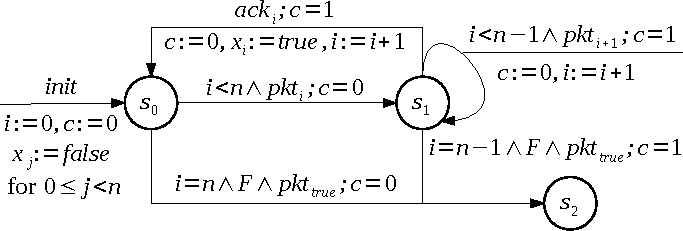
\includegraphics[width=0.7\textwidth]{sat_sm.pdf}
    \caption{\textbf{Monitor State Machine for SAT Problem.}}
    \label{fig:sat}
  \end{figure}



  The protocol monitor state machine $S$ is shown in Fig.~\ref{fig:sat}.
  Initially, all $x_i$ is set to \texttt{false}.
  At state $s_0$, the DUT shall transmit $pkt_i$ within a unit time, transit to
  $s_1$ and reset the clock along the transition.
  At state $s_1$, either the DUT receives the $ack_i$ packet and
  set $x_i$ to be \texttt{true} ($s_1 \rightarrow s_0$), or the DUT continues to
  transmit the next packet $pkt_{i+1}$.
  After $n$ rounds, the state machine is $s_0$ or $s_1$ depending on whether
  $ack_{n-1}$ is received by the DUT.
  In either case, the DUT shall evaluate $F$ and transmit $pkt_{true}$ if $F$ is
  \texttt{true}.  

  \sloppy{    Consider a sniffer trace $Tr_1=\{(0, pkt_0), (2, pkt_1), (4, pkt_2),\ldots,
  (2(n-1), pkt_{n-1}), (2n, pkt_{true})\}$.  That is, the sniffer only captures
  all $pkt_i$ plus the final $pkt_{true}$, but none of $ack_i$.  It is easy to see
  that $F$ is satisfiable if $S_1^+$ accepts $Tr_1$.  In particular, a successful
  run of $S_1^+$ on $Tr_1$ would have to guess, for each $pkt_i$, whether the
  Type-1 empty transitions should be used to infer the missing $ack_i$ packet,
  such that $F$ is \textit{true} at the end.  Note that for $Tr_1$, no Type-2 self
  transitions can be used since all packets in $Tr_1$ are sent from the DUT.
  Therefore, the SAT problem of $F$ can be reduced to the VALIDATION-1 problem of
  $S^+_1$ on sniffer trace $Tr_1$.
  }

  \sloppy{    On the other hand, consider another sniffer trace $Tr_2 =\{(0, pkt_0), (1,
    ack_0), (2, pkt_1), (3, ack_1),\ldots, (2n-2, pkt_{n-1}), (2n-1, ack_{n-1}),\\ (2n,
  pkt_{true}\}$. That is, the sniffer captures all $n$ pair of $pkt_i$ and $ack_i$
  packets and the final $pkt_{true}$ packet.  Similar to $Tr_1$, $F$ is
  satisfiable if $S^+_2$ accepts $Tr_2$. A successful transition sequence of
  $S^+_2$ on $Tr_2$ must decide for each $ack_i$ packet, whether Type-2 self
  transitions should be used, so that $F$ can be evaluated as true at the end.
  Therefore, the SAT problem of $F$ can also be reduced to the VALIDATION-2
  problem of $S^+_2$ on sniffer trace $Tr_2$.
}

Since SAT is known to be NP-complete, both the VALIDATION-1 and the
VALIDATION-2 problem are also NP-complete.  \qed
\end{proof}

The hardness statement of the general VALIDATION problem naturally follows
Lemma~\ref{lem:sub}.

\begin{theorem}
  VALIDATION is NP-complete.
\end{theorem}
 
\makeatletter{}\subsection{Searching Strategies}
\label{subsec:search}

In this section, we present an \textit{exhaustive} search algorithm of the
accepting transition sequence of $S^+$ on sniffer trace $Tr$. It is guaranteed to
yield an accepting sequence if there exists one, thus is exhaustive.  In the next
sections, we present heuristics to limit the search to accepting sequences of
$S^+$ that require relatively fewer transitions from $E^+_1 \cup E^+_2$.  Due to
the NP-completeness of the problem, this also makes the algorithm meaningful in
practice.

\begin{figure}[t!]
  \begin{minipage}{\textwidth}
    \begin{algorithm}[H]
      \caption{Exhaustive search algorithm of $S^+$ on $Tr$.}
      \label{alg:search}
      
      \begin{algorithmic}[1]
        \Function{search}{S, Tr}
          \Let{$S^+$}{\Call{augment}{S}}
          \State\Return{\Call{extend}{[], Tr, $S^+.s_0$}}
        \EndFunction
        \Function{extend}{prefix, p::suffix, $s$}
          \If{not \Call{likely}{prefix}}
            \label{alg:search:stop}
            {\Return{\nil}}\footnote{This check should be ignored in the exhaustive algorithm.}
          \EndIf
          \For{i $\in$ [0, 1, 2]}
          \label{alg:search:order}
          \Let{mutation}{EXTEND-i(prefix, p::suffix, $s$)}
            \If{mutation $\ne$ \nil}
              {\Return{mutation}}
            \EndIf
          \EndFor
          \State\Return{\nil}
        \EndFunction
        \Function{extend-0}{prefix, p::suffix, $s$}
          \For{$\langle s, s', p\rangle\footnote{$\langle s, s', p \rangle$ is
              short for $\langle s, *, s', *, p, *, *\rangle$} \in E$}
            \If{suffix = \nil}
              {\Return{prefix@p}}
              \label{alg:search:terminate_0}
            \EndIf
            \Let{mutation}{\Call{extend}{prefix@p, suffix, $s'$}}
            \label{alg:search:append}
            \If{mutation $\ne$ \nil}
              {\Return{mutation}}
            \EndIf
          \EndFor
          \State{\Return{\nil}}
        \EndFunction
        \Function{extend-1}{prefix, p::suffix, $s$}
          \ForAll{$\langle s, s', q\rangle \in E^+_1$}
            \If{q.time $>$ p.time}
              \label{alg:search:type_1_limit}
              \State{\textbf{continue}}
            \EndIf
            \Let{mutation}{\Call{extend}{prefix@q, p::suffix, $s'$}}
            \label{alg:search:guess}
            \If{mutation $\ne \nil$}
              {\Return{mutation}}
            \EndIf
          \EndFor
          \State{\Return{\nil}}
        \EndFunction
        \Function{extend-2}{prefix, p::suffix, $s$}
          \ForAll{$\langle s, s, p \rangle \in E^+_2$}
            \If{suffix = \nil}
              {\Return{prefix}}
              \label{alg:search:terminate_2}
            \EndIf
            \Let{mutation}{\Call{extend}{prefix, suffix, $s$}}
            \label{alg:search:drop}
            \If{mutation $\ne$ \nil}
              {\Return{mutation}}
            \EndIf
          \EndFor
          \State{\Return{\nil}}
        \EndFunction
      \end{algorithmic}
    \end{algorithm}
    \renewcommand\footnoterule{}
  \end{minipage}
\end{figure}

The main routines of the algorithm are shown in Algorithm~\ref{alg:search}.  In
the top level \texttt{SEARCH} routine, we first obtain the augmented state
machine $S^+$, and then call the recursive \texttt{EXTEND} function with an empty
prefix, the sniffer trace, and the $S^+$'s initial state. 
In the \texttt{EXTEND} function, we try to consume the first packet in the
remaining trace using either Type-0, Type-1 or Type-2 transition.
Note that we always try to use Type-0 transitions before other two augmented
transitions (line~\ref{alg:search:order}).
This ensures the first found mutation trace will have the most number of Type-0
transitions among all possible mutation traces.
Intuitively, this means the search algorithm tries to utilize the sniffer's
observation as much as possible before being forced to make assumptions.


Each of the extend functions either returns the mutation trace $Tr'$, or
\textit{\nil} if the search fails.
In both \texttt{EXTEND-0} and
\texttt{EXTEND-2} function, if there is a valid transition, we try to consume
the next packet either by appending it to the prefix
(line~\ref{alg:search:append}) or dropping it (line~\ref{alg:search:drop}).
While in \texttt{EXTEND-1}, we guess a missing packet without consuming the next
real packet (line~\ref{alg:search:guess}).
Note that since only Type-0 and Type-2 consume packets, the recursion terminates
if there is a valid Type-0 or Type-2 transition for the last packet
(line~\ref{alg:search:terminate_0} and line~\ref{alg:search:terminate_2}).



It is not hard to see that Algorithm~\ref{alg:search} terminates on any sniffer
traces. Each node in the transition tree only has finite number of possible next
steps, and the depth of Type-1 transitions is limited by the time available
before the next packet (line~\ref{alg:search:type_1_limit}).
 
\makeatletter{}\subsection{Pruning Heuristics}
\label{subsec:heuristic}

In the face of uncertainty between a possible
protocol violation and sniffer imperfection, augmented transitions provide the
ability to blame the latter. The exhaustive nature of
Algorithm~\ref{alg:search} means that it always tries to blame sniffer
imperfection whenever possible, making it reluctant to report true
violations.

Inspired by the \textit{directed model checking}~\cite{edelkamp2008survey}
technique which is to mitigate the state explosion problem, we propose to enforce extra
constraints on the mutation trace to restrict the search to only mutation traces
with high likelihood. The modified \texttt{EXTEND} function checks certain
likelihood constraints on the prefix of the mutation trace before continuing
(line~\ref{alg:search:stop}), and stops the current search branch immediately if
the prefix seems \textit{unlikely}.  Because of the recursive nature of the
algorithm, other branches which may have a higher likelihood can then be
explored.

The strictness of the likelihood constraint represents a trade-off between
precision and recall of validation. The more strict the constraints are, the
more false positive violations will potentially be reported, hence the lower the
precision yet higher recall. On the contrary, the more tractable the
constraints are, the more tolerant the search is to sniffer imperfection, hence
the more likely that it will report true violations, thus higher precision but
lower recall.

The exact forms of the constraints may depend on many factors, such as the
nature of the protocol, properties of the sniffer, or domain knowledge.  Next,
we propose two \textit{protocol oblivious} heuristics based on the sniffer loss
probabilities and general protocol operations. Both heuristic contains
parameters that can be fine tuned in practice.

\subsubsection{$\mathit{NumMissing}(d, l, k)$}

This heuristic states that the number of missing packets from device $d$ in any
sub mutation traces of length $l$ shall not exceed $k$ ($k \le l$).  The sliding
window of size $l$ serves two purposes. First, $l$ should be large enough for
the calculated packet loss ratio to be statistically meaningful.  Second, it
ensures that the packet losses are evenly distributed among the entire packet
trace.

The intuition behind this heuristic is that the sniffer's empirical packet loss
probability can usually be measured before validation. Therefore, the likelihood
that the sniffer misses more packets than prior measured loss ratio is quite
low. The value of $l$ and $k$ can then be configured such that $k/l$ is marginally
larger than the measured ratio.

\begin{comment}
In addition, we note that for a fixed $l$, a single threshold $k$ may not work
for traces collected by sniffers with different packet loss probabilities.
Intuitively, sniffers with high loss probabilities require a larger threshold.
Therefore, we perform a \textit{stratified} search with an increasing sequence
of thresholds $\{k_1, k_2,\ldots, k_n\}$ ($k_i < k_{i+1}$ for $1 \le i < n$).
At round $i$, the search is restricted by constraint $NumMissing(d, l, k_i)$.
If a mutation trace is found, the search is completed.  Otherwise, we increase
the round number and repeat the search process.  In this way, this heuristic can
automatically adapt to the underlying sniffer packet loss probabilities. And a
violation is declared when no mutation trace can be found with $NumMissing(d, l,
k_n)$.
\end{comment}

\subsubsection{$\mathit{GoBack}(k)$}

This heuristic states that the search should only
backtrack at most $k$ steps when the search gets stuck using only $E$.
The motivation is that many protocols operate as a sequence of independent
transactions, and the uncertainty of previous transactions often do not affect
the next transaction.
For instance, in 802.11 packet transmission protocol, each packet exchange,
include the original, retransmission and acknowledgment packets, constitute a
transaction.
And the retransmission status of previous packets has no effect on the packets
with subsequent sequence numbers, hence need not be explored when resolving the
uncertainty of the packets with new sequence numbers.  Note that we do not
require the protocol to specify an exact transaction boundary, but only need $k$
to be sufficiently large to cover a transaction. 

\begin{comment}
\subsection{Confidence of Correctness}

A run of $S^+$ on sniffer packet trace $Tr$ may yield two conclusions about the
DUT implementation: either ``definitely wrong'' when $S^+$ rejects $Tr$, or
``possibly correct'' when $S^+$ accepts $Tr$. We now quantify the
\textit{confidence} of the implementation correctness in the later case.

Note that the augmented transitions in $S^+$ implicitly embed the assumptions
about packet losses. In particular, Type-1 transitions assume the sniffer
missed certain packets, while Type-2 transitions assume the sniffer
overheard packets that were missed by the DUT. Intuitively, the portion of such
assumptions (hence packet loss \textit{ratios}) in an accepting transition
sequence should match with the true packet loss \textit{probabilities}.
Otherwise, the correctness confidence, despite $S^+$ accepts $Tr$, is low.

Suppose $Tr$ is the sniffer trace and $Tr'$ is its mutation that satisfies $S$.
We can calculate the three packet loss ratios in our model shown in
Figure~\ref{fig:prob}.

\begin{align}
  &Pr_{ds} = \frac{\parallel \{(t,p) \in Tr'\setminus Tr \land p.src = DUT\}\parallel}
  {\parallel \{(t,p) \in Tr' \cup Tr \land p.src = DUT\}\parallel}\\
  &Pr_{es} = \frac{\parallel \{(t,p) \in Tr'\setminus Tr \land p.src = EP\}\parallel}
  {\parallel \{(t,p) \in Tr' \cup Tr \land p.src = EP\}\parallel}
\end{align}where $Tr'\setminus Tr$ is the set of inferred packets that were missed by the
sniffer (Type-1 transitions in $S^+$).

Note that we can not directly calculate the packet loss ratio from Endpoint to
DUT, since there might be packets that were missed by both the sniffer and the
DUT. We can, however, approximate $Pr_{ed}$ using conditional packet loss
probability.

\begin{align}
  \nonumber
  &(1-Pr_{es})\times Pr_{ed} =\\
  &\frac{\parallel \{(t,p) \in Tr\setminus Tr' \land p.src = EP \land p.dest = DUT\}\parallel}
  {\parallel \{(t,p) \in Tr \cup Tr' \land p.src = EP \land p.dest = DUT\}\parallel}
\end{align}The LHS is the probability that a packet sent from the Endpoint to the DUT was
missed by the DUT yet captured by the sniffer. And the RHS is the ratio of
such packets in the mutation trace.


Consider the 802.11 data transmission protocol and the example trace snippet
shown in Figure~\ref{fig:loss}, the packet loss ratios are:
\begin{align*}
  Pr_{ds} &= \frac{\parallel\{\it{DATA}'_0\}\parallel}{\parallel\{\it{DATA}_0, \it{DATA}'_0\}\parallel} = 0.5\\
  Pr_{es} &= \frac{\parallel\emptyset\parallel}{\parallel\{Ack, Ack\}\parallel} = 0\\
  Pr_{ed} &= \frac{\parallel\{Ack\}\parallel}{\parallel\{Ack, Ack\}\parallel\times (1-Pr_{es})} = 0.5
\end{align*}

\begin{figure}[t!]
  \centering
  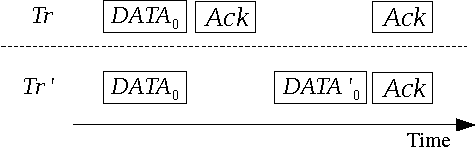
\includegraphics[width=0.4\textwidth]{loss.pdf}
  \caption{\textbf{Example Sniffer Trace and Its Mutation Trace.}}
  \label{fig:loss}
\end{figure}

Suppose we have the true packet loss probabilities $\overline{Pr_{ds}},
\overline{Pr_{es}}$ and $\overline{Pr_{ed}}$, the \textit{confidence} of this
mutation trace $Tr'$ can be defined as:

\begin{align}
  Confidence(Tr') = \prod_{i\in\{ds, es, ed\}}(1-|Pr_i-\overline{Pr_i}|)
\end{align}

By this definition, the trace confidence maximizes when all packet loss
ratios calculated from $Tr'$ matches the true packet
loss probabilities.

Suppose we have $M$ mutation traces that satisfies $S$, then
the overall \textit{confidence of correctness} from sniffer trace $Tr$ can be defined as:

\begin{align}
  Confidence(Tr) &= 1-\prod_{j=1}^{M}(1-Pr(Tr'_j))
\end{align}

Since $0 \le 1-Pr(Tr'_j) \le 1$ for all $j$, we have:

\begin{align}
  \nonumber
  Confidence(Tr) &\ge 1-(1-Pr(Tr'_j)\\
     &= Pr(Tr'_j)
\end{align}for all $j$.

This means if we can find a mutation trace $Tr'$ that satisfies $S$, then the
overall confidence of the correctness is no less than $Pr(Tr')$.
\end{comment}
 
 
\makeatletter{}\section{Case Studies}
\label{sec:case}

We present case studies on applying our validation framework on two protocols
implemented in the \ns{} network simulator: 802.11 data transmission and ARF
rate control algorithm. The goal is to demonstrate how our framework can avoid
false alarms and report true violations on incomplete sniffer traces and report
true violations. We also report the application of our framework to a commercial
product under development.

\makeatletter{}\subsection{802.11 Data Transmission}
\label{subsec:tx}

In this section, we first show that our framework can improve validation
precision by inferring the missing or extra packets using the augmented
transition framework. We then demonstrate the ability of our framework to detect
true violations by manually introducing bugs in the \ns{} implementation and
show the precision and recall of validation results.


\subsubsection{Experimental Setup}

We set up two \wifi{} devices acting as the transmitter (DUT) and receiver
respectively. Another \wifi{} device is configured in monitor mode and acts as
the sniffer. During the experiments,we collect both the DUT packet trace
(the ground truth) and the sniffer trace.

\subsubsection{Verifying Unmodified Implementation}

In the original monitor state machine shown in Fig.~\ref{fig:dot11_tx_ta}, we
set acknowledgment timeout $T_o=334\mu$s, maximum retransmission delay
$T_m=15$ms according to the protocol. We also adapt the state machine to include
multiple retransmissions\footnote{The exact number of retransmissions is not
part of the protocol, and NS-3 implementation set this to be 7.} instead of one.

Let $Pr_{ds}$, $Pr_{es}$ and $Pr_{ed}$ be the packet loss probability between
the DUT and sniffer, endpoint and sniffer, endpoint and DUT respectively.
$Pr_{ed}$ represents the characteristics of the system being tested, while
$Pr_{ds}$ and $Pr_{es}$ represent the sniffer's quality in capturing packets.



We vary each of the three probabilities, $Pr_{ds}$, $Pr_{es}$ and $Pr_{ed}$, from
0 to 0.5 (both inclusive) with 0.05 step.  For each loss ratio combination, we
ran the experiment 5 times, and each run lasted
30 seconds. In total, 6655 ($11^3\times 5$) pairs of DUT and sniffer packet
traces were collected.

To establish the ground truth of violations, we first verify the DUT packet
traces using the \textit{original} state machine $S$.  This can be achieved by
disabling augmented transitions in our framework.  As expected, no violation is
detected in any DUT packet traces.

We then verify the sniffer traces using the augmented state machine $S^+$.  For
the $\mathit{GoBack}(k)$ heuristic, we set $k=7$, which is the maximum number of
transmissions of a single packet. For the $\mathit{NumMissing}(d, l, k)$ heuristic, we
set the sliding window size $l=100$, and $k=80$ such that no violation is
reported. The relationship of $k$ and validation precision is studied in next
section.

Next, we present detailed analysis of the augmented transitions on the sniffer
traces. The goal is to study for a given system packet loss probability
$Pr_{ed}$, how the sniffer packet loss properties ($Pr_{ds}$ and $Pr_{es}$)
affect the difference between the DUT trace and the mutation trace, which represents
a guess of the DUT trace by the augmented state machine based on the sniffer
trace.

For all following analysis, we divide the traces into three groups according to
$Pr_{ed}$: low ($0 \le Pr_{ed} \le 0.15$), medium ($0.20 \le Pr_{ed} \le 0.35$)
and high ($0.40 \le Pr_{ed} \le 0.50$).

The different between two packet traces can be quantified by the Jaccard distance
metric.

\begin{align}
  Jaccard(Tr_1, Tr_2) = \frac{\left\vert Tr_1 \ominus Tr_2\right\vert}{\left\vert
  Tr_1 \cup Tr_2\right\vert}
\end{align}where $\ominus$ is the symmetric difference operator.  The distance is 0 if the
two traces are identical, and is 1 when the two traces are completely different.
The smaller the distance is, the more similar the two traces are.

A na\"ive way to calculate the Jaccard distance of two traces is to use the hash
of the $(time, packet)$ pair for set intersection and union operation.  However,
it does not work for mutation trace which contains fabricated packets with no
actual payload.  Therefore, we use a protocol specific canonical representation
of packets when calculating the distance.  In particular, the string
\texttt{r\_\it{DATA}\_i\_t} represents the $t^{th}$ transmission of a data packet
with sequence number $i$, and $r$ represents the round of sequence numbers as it
wraps after 4096.  And similarly \texttt{r\_Ack\_i\_t} is the corresponding
acknowledgment packet.

\begin{figure*}[t!]
  \centering
  \begin{subfigure}{0.33\textwidth}
    \centering
    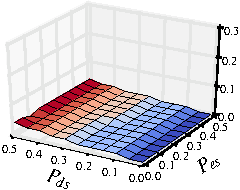
\includegraphics[width=\textwidth]{MutationDUTJaccard3DFigure_0_10.pdf}
        \caption{$0.05 \le Pr_{ed} \le 0.15$}
  \end{subfigure}\hspace*{0.01\textwidth}
  \begin{subfigure}{0.33\textwidth}
    \centering
    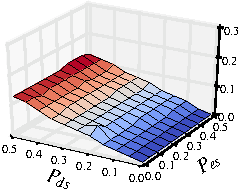
\includegraphics[width=\textwidth]{MutationDUTJaccard3DFigure_0_30.pdf}
    \caption{$0.2 \le Pr_{ed} \le 0.35$}
  \end{subfigure}\hspace*{0.01\textwidth}
  \begin{subfigure}{0.33\textwidth}
    \centering
    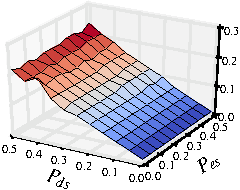
\includegraphics[width=\textwidth]{MutationDUTJaccard3DFigure_0_50.pdf}
    \caption{$0.4 \le Pr_{ed} \le 0.5$}
  \end{subfigure}\hspace*{0.01\textwidth}
  \caption{\textbf{Jaccard Distance Between Mutation and DUT Traces.} For each
  data point, the mean of the 5 runs is used.}
  \label{fig:mutation_dut}
\end{figure*}


Fig.~\ref{fig:mutation_dut} shows the Jaccard Distance between mutation and its
corresponding DUT trace. We make the following observations. First, for a given
system loss probability $Pr_{ed}$ (each sub-figure), the lower the sniffer
packet loss probability ($Pr_{ds}$ and $Pr_{es}$), the smaller Jaccard distance
between the DUT and mutation trace. Intuitively, this means a sniffer that
misses less packets can enable our framework to better reconstruct the DUT
trace.

Second, we observe a \textit{protocol-specific} trend that $Pr_{ds}$ is more
dominant than $Pr_{es}$.  This is because retransmission packets of the same
sequence number are identical, hence when the sniffer misses multiple
retransmission packets, our framework only needs to infer one retransmission
packet to continue state machine execution.

Finally, as the system loss probability $Pr_{ed}$ increases, the Jaccard
distance increases more rapidly as $Pr_{ds}$ increases.  This is because the
ratio of retransmission packet increases along with $Pr_{ed}$.


We then evaluate the cost of resolving uncertainty. In particular, we use
the Average Search Steps Per Packet (ASSPP) as a metric to quantify the search
cost.  It is calculated by dividing the total number of search steps by the
number of packets in the packet trace. For DUT traces, ASSPP is always 1 since
there is no uncertainty. For sniffer traces, however, multiple search steps must
be to conducted to resolve the potential uncertainty of each packet in the
sniffer trace.

\begin{figure*}[t!]
  \centering
  \begin{subfigure}{0.33\textwidth}
    \centering
    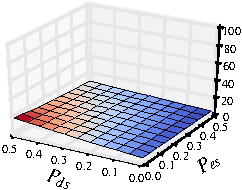
\includegraphics[width=\textwidth]{StepCount3DFigure_0_10.pdf}
    \caption{$Pr_{ed} \in [0.05, 0.10, 0.15]$}
  \end{subfigure}\hspace*{0.01\textwidth}
  \begin{subfigure}{0.33\textwidth}
    \centering
    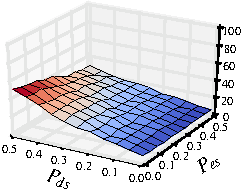
\includegraphics[width=\textwidth]{StepCount3DFigure_0_30.pdf}
    \caption{$Pr_{ed} \in [0.2, 0.25, 0.3, 0.35]$}
  \end{subfigure}\hspace*{0.01\textwidth}
  \begin{subfigure}{0.33\textwidth}
    \centering
    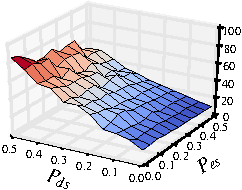
\includegraphics[width=\textwidth]{StepCount3DFigure_0_50.pdf}
    \caption{$Pr_{ed} \in [0.40, 0.45, 0.50]$}
  \end{subfigure}
  \caption{\textbf{Average Searching Step Per Packet.} For each data point, the mean of 5 runs
  is used.}
  \label{fig:cost}
\end{figure*}


Fig.~\ref{fig:cost} shows the distribution of ASSPP at different $Pr_{ed}$.
Similar to the case in Fig.~\ref{fig:mutation_dut}, $Pr_{ds}$ plays a dominant
role in determine the searching cost. One interesting observation for this
particular protocol is that the
search cost peaks when $Pr_{ds}$ is high while $Pr_{es}$ is low. In such loss
probability combinations, sniffer misses many data packets from the DUT but
picks up lots of \textit{dangling} $Ack$ packets from the DUT. Because the $Ack$
packet has neither sequence numbers nor retry flag, the searching algorithm had
a hard time resolving such uncertainty.

\subsubsection{Introducing Bugs}

We have demonstrated that our framework can tolerate sniffer imperfections and
avoid raising false alarms.  The next question is, can it detect true
violations?  To answer this question, we manually introduce several bugs in
\ns{} implementation that concerns various aspects of 802.11 data transmission
protocol.  More specifically, the bugs are:

\begin{itemize}
  \item \textbf{Sequence Number}: the DUT does not assign sequence number
    correctly. For example, it may increase sequence by 2 instead of 1, or it
    does not increase sequence number after certain packet, etc. We choose one
    type of such bugs in each run.
  \item \textbf{Semantic}: the DUT may retransmit even
    after receiving $Ack$, or does not retransmit when not receiving $Ack$.
\end{itemize}

We instrument the \ns{} implementation to embed instances of bugs in each
category. At each experiment run, we randomly decide whether and which bug to
introduce for each category. We fix $Pr_{ds}=Pr_{es}=0.1$ and vary $Pr_{ed}$
from 0.0 to 0.5 with 0.01 step. For each $Pr_{ed}$ value, we ran the experiment
100 times, of which roughly 75 experiments contained bugs. In total, 5100 pairs of
DUT and sniffer traces were collected.


We use the DUT packet traces as ground truth of whether or not each experiment
run contains bugs.
For each $Pr_{ed}$ value, we calculate the precision and recall of violation
detection using the sniffer traces.\begin{align}
  \text{Precision} = \frac{\left\vert \{\text{Reported Bugs}\} \cap \{\text{True Bugs}\}\right\vert}{\left\vert
  \{\text{Reported Bugs}\}\right\vert}\\
  \text{Recall} = \frac{\left\vert \{\text{Reported Bugs}\} \cap \{\text{True Bugs}\}\right\vert}{\left\vert
  \{\text{True Bugs}\}\right\vert}
\end{align}The precision metric quantifies how \textit{useful} the validation results are ,
while the recall metric measures how \textit{complete} the validation results
are.

\begin{figure}[t!]
  \centering
  \begin{subfigure}{0.48\textwidth}
    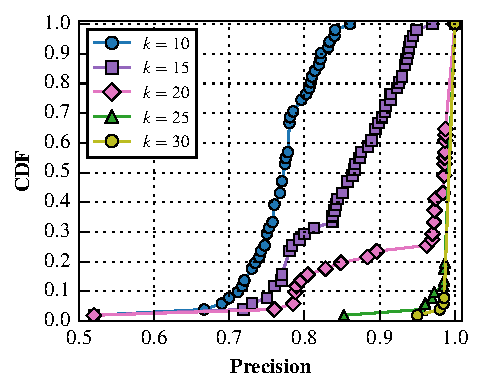
\includegraphics[width=\textwidth]{PrecisionFigure.pdf}
  \end{subfigure}
  \begin{subfigure}{0.48\textwidth}
    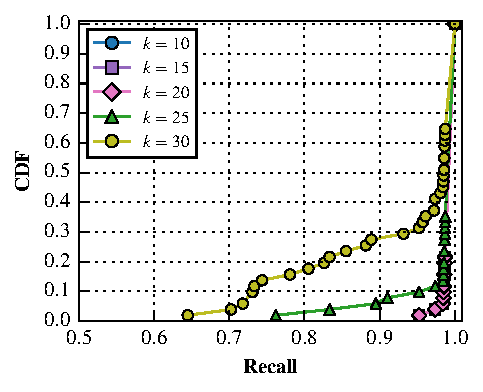
\includegraphics[width=\textwidth]{RecallFigure.pdf}
  \end{subfigure}
  \caption{\textbf{Precision and Recall of Validation Results.}}
  \label{fig:precision}
\end{figure}

Fig.~\ref{fig:precision} shows the CDF of precision and recall of the 51
experiments for various $k$ values. For precision, as expected, the more
tolerant the search to sniffer losses (larger $k$), the more tolerant the
framework is to sniffer losses, and the more precise the violation detection. In
particular, when $k=30$, the precisions are 100\% for all $Pr_{ed}$ values.
Second, the recall is less sensitive to the choice of $k$.  Except for the
extreme case when $k=30$, all other thresholds can report almost all the
violations.
 
\makeatletter{}\subsection{ARF Rate Control Algorithm}
\label{subsec:arf}

Automatic Rate Fallback (ARF)~\cite{kamerman1997wavelan} is the first rate
control algorithm in literature. In ARF, the sender increases the bit rate after
$Th_1$ number of consecutive successes or $Th_2$ number of packets with at most
one retransmission. The sender decreases bit rate after two consecutive packet
failures or if the first packet sent after rate increase (commonly referred as
\textit{probing} packet) fails.

\sloppy{  Fig.~\ref{fig:arf_sm} shows the state machine $S$ for the packet trace
  collected at sender (DUT), where $\it{DATA}_i^r$ denotes a data packet
  with sequence number $i$ and bit rate $r$, $\it{DATA}_i^{r\prime}$ is a retransmission packet
  and $Ack$ is the acknowledgment packet. The \texttt{pkg\_succ} function is
  shown in Algorithm~\ref{alg:pkt_succ}.
}

\begin{figure}[t!]
  \centering
  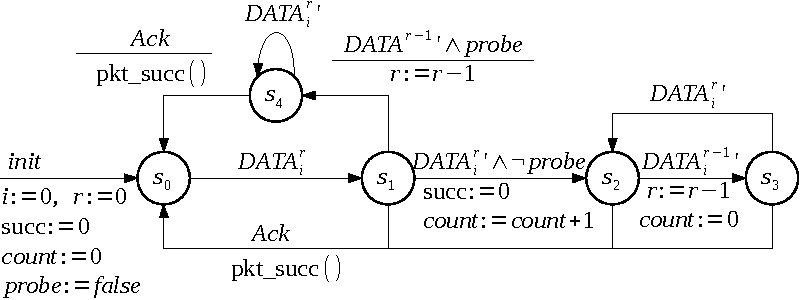
\includegraphics[width=0.8\textwidth]{arf_sm.pdf}
  \caption{\textbf{Monitor State Machine for ARF Rate Control Algorithm.} Timing
  constraints are omitted for succinctness.}
  \label{fig:arf_sm}
\end{figure}


The \texttt{succ} variable is used to track the number of consecutive packet
successes. It is increased after each packet success , and is reset to 0 after a
rate increase or upon a packet failure ($s_1\rightarrow s_2$).  Similarly,
\texttt{count} is to track the number of packets with at most one
retransmission, and is increased after packet success, or for the first packet
retransmission ($s_1\rightarrow s_2$). It is reset when there are two
consecutive packet failures ($s_2\rightarrow s_3$). Finally, the \texttt{probe}
flag is set upon rate increases to indicate the probing packet, and is cleared
upon packet success. The variable \texttt{r} is the current bit rate, which is
decreased if the probing packet fails ($s_1\rightarrow s_4$), or every two
consecutive failures ($s_2\rightarrow s_3$). If \texttt{r} is not the highest
rate, it is increased when either of the two thresholds are reached.


\begin{algorithm}[t!]
  \caption{\texttt{pkt\_succ} function}
  \label{alg:pkt_succ}
  \begin{algorithmic}[1]
    \Function{pkt\_succ}{}
    \Let{i}{(i+1)\%N}
    \Let{succ}{succ + 1}
    \Let{count}{count + 1}
    \Let{probe}{false}
    \If{r $< R$ and (succ $\ge Th_1$ or count $\ge Th_2$)}
    \Let{r}{r+1}
    \Let{succ}{0}
    \Let{count}{0}
    \Let{probe}{true}
    \EndIf
    \EndFunction
  \end{algorithmic}
\end{algorithm}

In particular, the bug we found lies in the implementation's \texttt{pkt\_succ}
function in line 6. Instead of checking \texttt{count $\ge$ Th\_2}, the
implementation checks \texttt{count == Th\_2}. This bug also exists in the NS-3
implementation of Adaptive ARF (AARF) algorithm~\cite{lacage2004ieee} and the
pseudo code implementation of AARF in~\cite{lacage2004report}.

Note that the \texttt{count} variable is incremented twice if a packet succeed
after one retransmission: once in $s_1\rightarrow s_2$, once in the
\texttt{pkt\_succ} function for the retransmission packet. Therefore, if the
value of \texttt{count} is $Th_2-1$ and the next packet succeed after one
retransmission, the value of \texttt{count} will be $Th_2+1$, which would fail
the implementation's test of \texttt{count == Th\_2}.

We report a bug found in NS-3 ARF~\cite{kamerman1997wavelan} implementation
which causes the sender to get stuck at a lower rate even after enough number of
consecutive successes. The bug was detected using sniffer traces and
confirmed by both the DUT trace and source code inspection.
 
\makeatletter{}\subsection{Industrial Application}
\label{subsec:xbox}

\begin{table}[t!]
  \centering
  \begin{tabular}{lll}
    \toprule
    \textbf{Protocol Aspects} & \textbf{Traces} & \textbf{Violations (\%)}\\
    \midrule
    Sequence Number & 3049 & 1539 (50.48\%) \\
    Station Scheduling & 3046 & 2045 (67.14\%) \\
    Uplink Modulation & 3127 & 8 (0.26\%) \\
    Downlink Modulation & 3127 & 24 (0.77\%) \\
    \bottomrule
  \end{tabular}
  \caption{\textbf{Validation Results on Traces from the Gaming Wireless Protocol.}}
  \label{tab:xbox}
\end{table}

We have applied our framework for runtime verification of the wireless protocol
implementation of a commercial product that has several millions of shipping
devices. The product runs a proprietary wireless protocol to reduce latency and
power consumption. Sniffer traces were collected in regular testing process, but
were only manually inspected previously. 

We obtained 75 sniffer traces from the testing team for a new version of the
protocol that is under development and testing. This team has been testing the
implementation for a few weeks.  Each trace contained around 6 million packets
that were captured during 1 hour and 40 minutes of protocol operation.

We split the traces into \num{100000} packet segments, and applied our framework
to validate the DUT implementation. We found that the latest implementation of
the protocol under development had violations of the protocol specification.
Some of the implementation bugs we found related to the sequence number
management, station scheduling during power saving mode, and modulation rates
adaptation.

Table~\ref{tab:xbox} summarizes the validation result. Note that if we disable
the augmented transitions, each trace will be flagged as violation because of
the missing packets, thereby reducing the usability of the tool. We also note
that some bugs manifest more often than others. For instance, the bugs related
to packet sequence number and station scheduler were detected in about half the
traces, and the bug related to the rate control algorithm was detected in only a
few traces. This is because the previous two aspects are essential in all
protocol operations, while the bugs related to rate control only manifest
themselves under certain link conditions.

After communicating with the testing team, we confirmed that the sequence number
bug was already known, as it is relatively easy to detect even by manually
examining the traces. The bug related to station scheduling was also noticed
before, yet no quantitative results about how frequent this bug appears were
obtained because of the lack of automatized validating tools. Finally, the bug
related to rate control has been filed as a bug report. All reported bugs were
fixed before the next release the product.
 
 
\makeatletter{}\section{Related Work}
\label{sec:related}

\textbf{Hidden Markov Model (HMM) Approach.} When considering the whole system
under test (both DUT and endpoint), the sniffer only captures a subset of the
all the packets (events).  This is similar to the event sampling problem in
runtime
verification~\cite{bonakdarpour2011sampling,hauswirth2004low,arnold2008qvm,fei2006artemis,basin2012monitoring}.
Stoller \textit{et al}~\cite{stoller2011runtime} used HMM-based state estimation
techniques to calculate the confidence that the temporal property is satisfied
in the presence of gaps in observation.

While it seems possible to adapt the
method in~\cite{stoller2011runtime} to our problem, we note several advantages
of our approach. First, the
automatically augmented state machine precisely encodes the protocol
specification and the uncertainty. This is intuitive to design and natural for
reporting the evidence for a trace being successful. We do not require a user
to specify the number of states of the underlying HMM, or accurately provide
underlying probabilities. Second, we use timed automata to monitor the timing
constraints which are common in wireless protocols. It may be non-trivial to
encode such timing information in HMM. Finally, we can exploit domain knowledge
to devise effective pruning heuristics to rule out unlikely sequences during the
exhaustive search. 

\textbf{Network Protocol Validation.} Lee \textit{et al}~\cite{lee1997passive}
studied the problem of passive network testing of network management. The system
input/output behavior is only partially observable. However, the uncertainty
only lies in missing events in the observation, while in the context of wireless
protocol verification, the uncertainty could also be caused by extra events not
observed by the tested system. Additionally, they do not provide any formal
guarantees even for cases when we report a definite bug.  Software model
checking techniques~\cite{musuvathi2002cmc,godefroid1997model} have also been
used to verify network protocols. Our problem is unique because of the
observation uncertainty caused by sniffers. Our framework shares similarity
with {\it angelic verification}~\cite{das-cav15} where the program verifier
reports a warning only when no acceptable specification exists on unknowns.

\begin{comment}
\textbf{Sniffer Trace Analysis.} Wireless sniffers has been widely used to
analyze MAC layer behaviors of enterprise wireless
networks~\cite{sheng:wicom2008,tan:tmc2014,yeo-wise04,yeo:witmemo2005}.
Jigsaw~\cite{Cheng:2006:JSP:1159913.1159920} is a larger scale wireless network
monitoring infrastructure. 150~radio monitors were deployed in a campus
building. Traces collected from multiple sniffers were merged and synchronized
to restructure the link and transportation layer conversations. Protocol
specific heuristics were developed to infer the missing packets. The work
in~\cite{Mahajan:2006:AMB:1159913.1159923} shared the same idea of trace merging
with Jigsaw, but uses a FSM to infer packet reception. These works assume the
correctness of the protocol implementation in order to infer missing packets,
while we systematically encode the uncertainty of sniffer traces for
verification purpose.


\textbf{ Testing Under Uncertainty}. The position paper by Rosemblum \textit{et
al}~\cite{Elbaum:2014:KUT:2635868.2666608} contains excellent motivation for the
need to combat uncertainty foundationally when testing systems. McKinley
\textit{et al}~\cite{bornholt2014uncertain,sampson2014expressing} deals with checking
assertions in programs dealing with noisy data from sensors. Instead of checking
the truth or falsity of assertions, they model the probability distribution of
the assertion conditions and perform Monte-carlo based simulations to estimate
the probabilities. Our work can be seen as leveraging non-determinism to weaken
the specification logically to precisely define the problem complexity, and use
probabilities to guide the search for likely mutations.  Other works have used
sampling to find data-race bugs~\cite{marino2009literace}, and ensure that the
sampling does not lead to spurious alarms.
\end{comment}
 
\makeatletter{}\section{Conclusions}
\label{sec:conclusion}

We formally define the uncertainty problem in validating wireless protocol
implementations using sniffers. We describe a systematic augmentation of the
protocol state machine to explicitly encode the uncertainty of sniffer traces.
We characterize the NP-completeness of the problem and propose both an
exhaustive search algorithm and heuristics to restrict the search to more likely
traces. We present two case studies using \ns{} network simulator to demonstrate
how our framework can improve validation precision and detect real bugs. We also
report the application of our framework on a commercial product under
development.

Finally, we discuss a few challenges and future
directions.

\textbf{Verification Coverage.} Given a single sniffer trace, it is possible
that not all the states in the state machine are visited during the verification
process. For instance, a rate control state machine based on certain consecutive
packet losses patterns can not be verified if no such consecutive losses appear
in the sniffer trace. In general, given a protocol state machine, it is
challenging to extract the packet patterns for each state to be reached and to
alter the testing such that such patterns can be observed.

\textbf{Automated State Machine Construction.} We manually constructed the
protocol monitor state machines for the protocols studied in this paper based on
the source code, comments and documentation. The process involves lots of labor
effort and is time-consuming. A potential alternative is to automatically learn
the sketch of the monitor state machines from the sniffer traces. Domain
knowledge can then be leveraged to improve the sketch state machines.
 



{\footnotesize
  \bibliographystyle{abbrv}
  \begin{thebibliography}{10}

\bibitem{alur1994theory}
R.~Alur and D.~L. Dill.
\newblock A theory of timed automata.
\newblock {\em Theoretical computer science}, 126(2):183--235, 1994.

\bibitem{arnold2008qvm}
M.~Arnold, M.~Vechev, and E.~Yahav.
\newblock Qvm: an efficient runtime for detecting defects in deployed systems.
\newblock In {\em ACM Sigplan Notices}, volume~43, pages 143--162. ACM, 2008.

\bibitem{bahl2006enhancing}
P.~Bahl, R.~Chandra, J.~Padhye, L.~Ravindranath, M.~Singh, A.~Wolman, and
  B.~Zill.
\newblock Enhancing the security of corporate \wifi{} networks using {DAIR}.
\newblock In {\em Proceedings of the 4th international conference on Mobile
  systems, applications and services}, pages 1--14. ACM, 2006.

\bibitem{basin2012monitoring}
D.~Basin, F.~Klaedtke, S.~Marinovic, and E.~Z{\u{a}}linescu.
\newblock Monitoring compliance policies over incomplete and disagreeing logs.
\newblock In {\em International Conference on Runtime Verification}, pages
  151--167. Springer, 2012.

\bibitem{bonakdarpour2011sampling}
B.~Bonakdarpour, S.~Navabpour, and S.~Fischmeister.
\newblock Sampling-based runtime verification.
\newblock In {\em FM 2011: Formal Methods}, pages 88--102. Springer, 2011.

\bibitem{cheng2006jigsaw}
Y.-C. Cheng, J.~Bellardo, P.~Benk{\"o}, A.~C. Snoeren, G.~M. Voelker, and
  S.~Savage.
\newblock {\em Jigsaw: solving the puzzle of enterprise 802.11 analysis},
  volume~36.
\newblock ACM, 2006.

\bibitem{wifried}
M.~Ciabarra.
\newblock {WiFried: iOS 8 WiFi Issue}.
\newblock \url{https://goo.gl/KtRDqk}.

\bibitem{das-cav15}
A.~Das, S.~K. Lahiri, A.~Lal, and Y.~Li.
\newblock Angelic verification: Precise verification modulo unknowns.
\newblock In {\em Computer Aided Verification - 27th International Conference,
  {CAV} 2015, San Francisco, CA, USA, July 18-24, 2015, Proceedings, Part {I}},
  pages 324--342, 2015.

\bibitem{surface}
digitalmediaphile.
\newblock Windows 10 wifi issues with surface pro 3 and surface 3.
\newblock \url{http://goo.gl/vBqiEo}.

\bibitem{edelkamp2008survey}
S.~Edelkamp, V.~Schuppan, D.~Bo{\v{s}}na{\v{c}}ki, A.~Wijs, A.~Fehnker, and
  H.~Aljazzar.
\newblock Survey on directed model checking.
\newblock In {\em International Workshop on Model Checking and Artificial
  Intelligence}, pages 65--89. Springer, 2008.

\bibitem{fei2006artemis}
L.~Fei and S.~P. Midkiff.
\newblock Artemis: Practical runtime monitoring of applications for execution
  anomalies.
\newblock In {\em ACM SIGPLAN Notices}, volume~41, pages 84--95. ACM, 2006.

\bibitem{lollipop}
Gizmodo.
\newblock The worst bugs in android 5.0 lollipop and how to fix them.
\newblock \url{http://goo.gl/akDcvA}.

\bibitem{godefroid1997model}
P.~Godefroid.
\newblock Model checking for programming languages using verisoft.
\newblock In {\em Proceedings of the 24th ACM SIGPLAN-SIGACT symposium on
  Principles of programming languages}, pages 174--186. ACM, 1997.

\bibitem{iris}
Google.
\newblock Google contact lens.
\newblock \url{https://en.wikipedia.org/wiki/Google_Contact_Lens}.

\bibitem{hauswirth2004low}
M.~Hauswirth and T.~M. Chilimbi.
\newblock Low-overhead memory leak detection using adaptive statistical
  profiling.
\newblock In {\em Acm Sigplan Notices}, volume~39, pages 156--164. ACM, 2004.

\bibitem{kamerman1997wavelan}
A.~Kamerman and L.~Monteban.
\newblock Wavelan{\textregistered}-ii: a high-performance wireless lan for the
  unlicensed band.
\newblock {\em Bell Labs technical journal}, 2(3):118--133, 1997.

\bibitem{lacage2004ieee}
M.~Lacage, M.~H. Manshaei, and T.~Turletti.
\newblock {IEEE 802.11 rate adaptation: a practical approach}.
\newblock In {\em Proceedings of the 7th ACM international symposium on
  Modeling, analysis and simulation of wireless and mobile systems}, pages
  126--134. ACM, 2004.

\bibitem{lacage2004report}
M.~Lacage, M.~H. Manshaei, and T.~Turletti.
\newblock {IEEE 802.11 rate adaptation: a practical approach}.
\newblock {\em [Research Report] RR-5208}, (<inria-00070784>):25, 2004.

\bibitem{lee1997passive}
D.~Lee, A.~N. Netravali, K.~K. Sabnani, B.~Sugla, and A.~John.
\newblock Passive testing and applications to network management.
\newblock In {\em Network Protocols, 1997. Proceedings., 1997 International
  Conference on}, pages 113--122. IEEE, 1997.

\bibitem{mahajan2006analyzing}
R.~Mahajan, M.~Rodrig, D.~Wetherall, and J.~Zahorjan.
\newblock Analyzing the mac-level behavior of wireless networks in the wild.
\newblock In {\em ACM SIGCOMM Computer Communication Review}, volume~36, pages
  75--86. ACM, 2006.

\bibitem{musuvathi2002cmc}
M.~Musuvathi, D.~Y. Park, A.~Chou, D.~R. Engler, and D.~L. Dill.
\newblock {CMC}: A pragmatic approach to model checking real code.
\newblock {\em ACM SIGOPS Operating Systems Review}, 36(SI):75--88, 2002.

\bibitem{mytkowicz2008observer}
T.~Mytkowicz, P.~F. Sweeney, M.~Hauswirth, and A.~Diwan.
\newblock Observer effect and measurement bias in performance analysis.
\newblock 2008.

\bibitem{riley2010ns}
G.~F. Riley and T.~R. Henderson.
\newblock The ns-3 network simulator.
\newblock In {\em Modeling and Tools for Network Simulation}, pages 15--34.
  Springer, 2010.

\bibitem{omnipeek}
{Savvius Inc.}
\newblock Savvius \wifi{} adapters.
\newblock \url{https://goo.gl/l3VXSx}.

\bibitem{Shi2016}
J.~Shi, S.~K. Lahiri, R.~Chandra, and G.~Challen.
\newblock {\em Wireless Protocol Validation Under Uncertainty}, pages 351--367.
\newblock Springer International Publishing, Cham, 2016.

\bibitem{stoller2011runtime}
S.~D. Stoller, E.~Bartocci, J.~Seyster, R.~Grosu, K.~Havelund, S.~A. Smolka,
  and E.~Zadok.
\newblock Runtime verification with state estimation.
\newblock In {\em Runtime Verification}, pages 193--207. Springer, 2011.

\bibitem{chromecast}
Wikipedia.
\newblock {Chromecast}.
\newblock \url{https://en.wikipedia.org/wiki/Chromecast}.

\bibitem{xbox}
Wikipedia.
\newblock {Xbox One} controller.
\newblock \url{https://en.wikipedia.org/wiki/Xbox_One_Controller}.

\end{thebibliography}
 
}


\end{document}
